\documentclass[a4paper, 12pt]{article}
\usepackage[left=30mm, top=25mm,right = 25mm, bottom=25mm]{geometry}
\usepackage{color}
\usepackage{url}
\usepackage[T2A]{fontenc} % enable Cyrillic fonts
\usepackage[utf8]{inputenc} % make weird characters work
\usepackage{graphicx}
\usepackage{tabularx}
\usepackage[english,serbian]{babel}
%\usepackage[english,serbianc]{babel} %ukljuciti babel sa ovim opcijama, umesto gornjim, ukoliko se koristi cirilica
\usepackage[OT1]{fontenc}
\usepackage[unicode]{hyperref}
\usepackage{amsmath}
\graphicspath{ {./images/} }
\hypersetup{colorlinks,citecolor=green,filecolor=green,linkcolor=blue,urlcolor=blue}

%\newtheorem{primer}{Пример}[section] %ćirilični primer
\newtheorem{primer}{Primer}[section]

\begin{document}

\title{\textbf{Stiven Hoking}\\ \small{Seminarski rad u okviru kursa\\Tehničko i naučno pisanje\\ Matematički fakultet}}

\author{
 \textbf {Lazar Rajčić}\\
  \text{lazarrajcic23@gmail.com}
  \and
  \textbf {Ivana Milenković}\\
  \text{ivanamilenkovic003@gmail.com}
  \and
 \textbf {Andjela Spasić}\\
  \text{spasic.andjela2013@gmail.com}
  \and
 \textbf {Nikola Stanojević}\\
  \text{nikola.stanojevic1903@gmail.com}
}
\date{14.~novembar 2022.}
\maketitle

\abstract{
Razlog zašto smo izabrali da pišemo o Stivenu Hoking-u jeste da bi ljudima približili njegove doprinose nauci uprkos barijerama koje je predstavljala njegova bolest. Unutar ovog seminarskog smo ispričali kratko njegovu životnu priču i objasnili neke od njegovih teorija.  

\tableofcontents

\newpage

\section{Uvod}
\label{sec:uvod}
Pre nego sto počnemo sa pričom o životu Stivena Hokinga i njegovim dostignućima moramo napraviti mali uvod u to ko je zapravo Stiven Hoking.
Stiven Hoking je bio engleski teoretski fizičar i kozmolog. Zbog njegovih doprinosa fizici smatran je za jednog od najvecih naučnika svog vremena. Njegovi doprinosi fizici se uglavnom nalaze u domenu našeg poznavanja crnih rupa ali o tome ćemo detaljnije pisati u zaglavlju Karijera. Zbog ovoga smatramo da je jako važno približiti njegova dostignuća ljudima.
Tematika ovog seminarskog rada je život i dostignuća Stivena Hokinga. Manja zaglavlja seminarskog su: Život, koji se dalje deli na život pre i posle dijagnoze, i Karijera.

\section{Život}
\subsection{Život pre dijagnoze i dijagnoza (rani život)}
Hoking se rodio 8. Januara 1942. Godine, tačno na tristotu godišnjicu smrti njegove 
velike inspiracije Galilea Galileja. Iako iznenđujuće nije bio najbolji ucenik, 
Stivena je od ranih nogu izuzetno interesovalo kako univerzum funkcioniše. Čak će u 
kasnijim godinama reći da ako razumemo kako univerzum radi mozemo u neku ruku i da ga 
kontrolišemo. Ova znatiželja koja će ga kasnije u životu gurati u napredovanju kariere,
u školi mu je zaslužila nadimak Ajnštajn. Planovi za dalje studiranje matematike 
ometeni su od strane njegovog oca koji je smatrao da u tome nema budućnosti. Usledio 
je kompromis, kojim je odlučeno da će Stiven da pohađa osnovne studije na polju fizike
na Oksfordu. Osnovne studije je zavrsio 1962. godine sa diplomom prvog reda posle 
čega se uputio na dalje obrazovanje na Kembridž univerzitetu. \medskip

Pri početku svojih studija na Kembridž-u Stiven je primetio da nesto nije sasvim u 
redu. Postao je vise trapav i imao je poteskoce sa malim stvarima poput vezivanja 
pertli. Nakon incidenta na klizanju majka ga je odvela u bolnicu na testiranje. Ne 
dugo nakon njegovog 21-og rodjendana saznaje se da ima neizlečivu bolest. Ta bolest 
se ispostavilo da je amiotrofička lateralna skleroza (eng. Amyotrophic lateral 
sclerosis) skraćeno ALS. To je bolest koja napada motorne nerve i polako ih uništava, 
ali nema efekta na mozak. Tadašnji doktori su zaključili da neće živeti duže od još 
dve godine. Ova vest ga je očekivano demoralizovala. Medjutim ubrzo nalazi ponovnu 
inspiraciju u Vagnerovoj muzici i ljubavi prema Džejn Vajld, svojoj buducoj supruzi. 
Kako je sada imao za koga da zivi, Stiven se ponovo bacio u svoja istraživanja koja 
su mu se, na sopstveno iznenadjenje, jako dopala. 

\begin{figure}[h!]
\centering
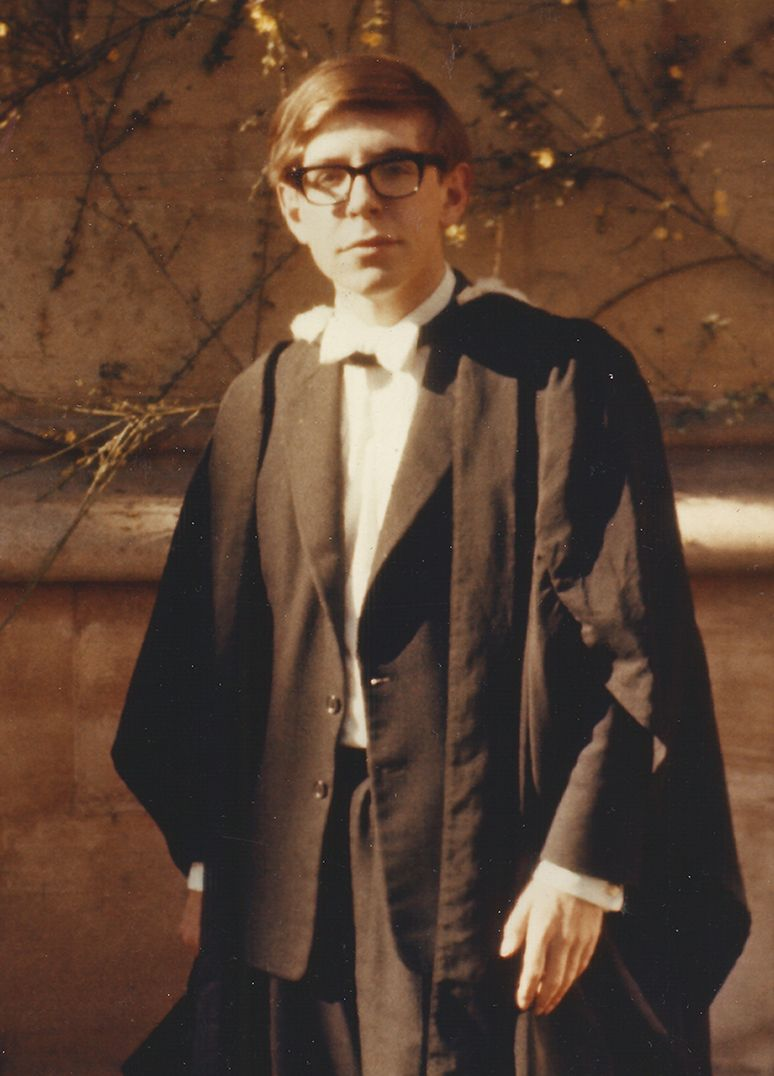
\includegraphics[width=0.5\textwidth]{Hoking,PreDijagnoze.jpg}
\caption{Hoking, na dodeli diploma 1960.}
\end{figure}

\subsection{Život nakon dijagnoze}
Iako je otpočeo karijeru sa puno entuzijazma, njen tok je bio dosta nepredvidljiv. 
Na Kembridž-u nije uspeo da nastavi studije pod Fredom Hojlom, u to doba izuzetno 
uglednim astronomom, kao sto je bila njegova zelja, jer je Hojl već imao previše 
studenata tada. Karijeru je zato otpočeo pod fizičarom i kozmologom Denisom Škiamom. 
Na ovo u kasnijim godinama Stiven gleda kao vrlo srećnu okolnost, koja je postavila 
temelje njegove dalje karijere. Govoreći takodje kako nije verovatno da bi dostigao 
veliki uspeh pod Hojlovim nadzorom. Ovo je potvrdila njihova javna prepirka 1964. 
godine, kada je Hoking prekinuo Hojlovo predavanje kako bi ukazao na grešku uglednog 
naučnika. \medskip
\newpage

Škiam ga je upoznao sa Rodžerom Penrouzom 1965. godine, sa kojim će kasnije sarađivati u nekim od svojih najvažnijih radova pri proučavanju crnih rupa. Te iste godine Hoking dobija doktorat i prijavljuje se za istraživačku stipendiju na univerzitetu u Kembridž-u. Ovo je pratio brak sa Dzejn Vajld, deca i napredak njegove kariere, ali i pogoršavanje bolesti. Bolest mu je uzela mogucnost hoda a kasnijem iz potrebe za hitnom traheotomijom i mogućnost govora. Komunikaciju je uspeo da održava preko mašine koja sintetiše govor. Mašinu je prvobitno koristio uz pomoć ručnog prekidača, a kasnije jednim misićem svog obraza. Preminuo je u udobnosti svog doma, 14. Marta 2018. godine. Uspeo je da preživi dijagnozu smrti do 23.-će godine  i doživi 76.-u godinu života.

\begin{figure}[h!]
\begin{center}
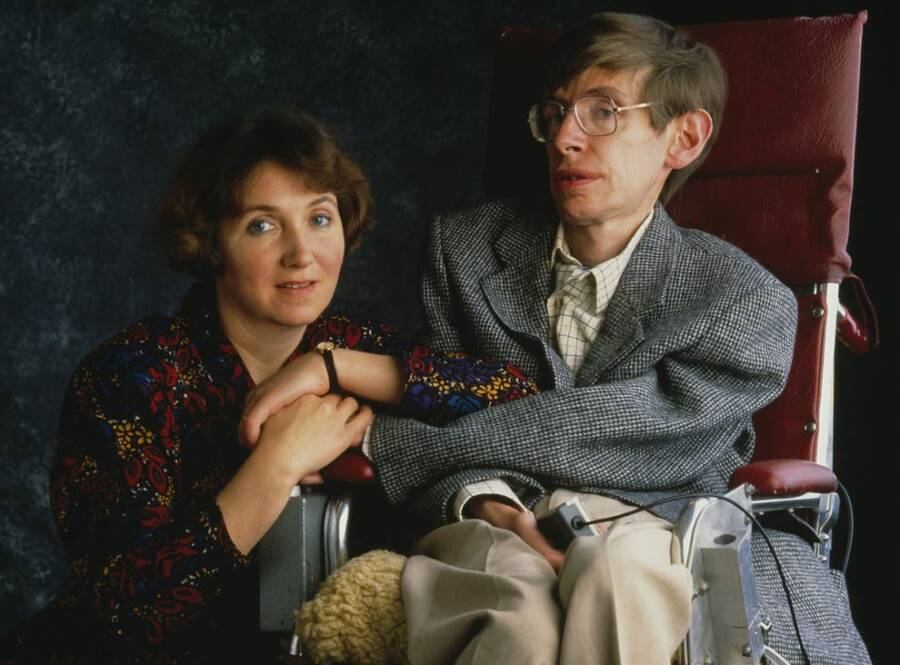
\includegraphics[width=1.0\textwidth]{StivenHoking.jpeg}
\end{center}
\caption{Stiven Hoking i njegova žena}
\label{fig:Stiven Hoking}
\end{figure}

\section{Karijera}
Karijera mu je otpočeta 1965. godine. Primarno je radio na poljima generalne relativnosti, posebno se interesujući za sferu crnih rupa. Prateći teoriju velikog praska, Hoking je, 1970. godine zajedno sa Rodzerom Penrouzom pokazao da ako se veliki prasak jeste desio i ako teorija relativiteta jeste istinita onda univerzum mora da je počeo iz tačke čija je zapremina nula ali koja je sadržala svu masu univerzuma. Prateći ovo 1971. godine izlaže teoriju postojanja objekata koje imaju masu biliona tona ali zauzimaju prostor jednog protona. Ovi objekti su nazvane male crne rupe. One nalažu svojom masom i gravitacijom da se na njih odnose zakoni klasične fizike, ali svojom veličinom da se odnose i zakoni kvantne fizike. Ovom teorijom nađena je veza između kvantne i klasične fizike, čije oktriće spada u jedno od Stivenovih najpoznatijih dela. Tri godine kasnije, 1974., izneo je teoriju, koja je kasnije potvrđena, da crne rupe emituju toplotno zračenje dok ne iscrpe svu svoju energiju, završavajući svoj život masivnom eksplozijom. Ova teorija se zove Hokingova radijacija. Ovo naravno nisu njegove jedine teorije, ali jesu najpoznatije.



\section{Karijera}
Osim toga što je bio teoretski fizičar i kosmolog, Hoking je takođe bio i autor, kao i član Kraljevskog društva (FRS), doživotni član Papeške akademije nauka, dobitnik predsedničke medalje o slobodi, najviše civilne nagrade u SAD-u. Hokingov doprinos fizici doneo mu je mnogo izuzetnih počasti. Postao je profesor gravitacione fizike na Kembridžu 1977. godine, a 1979. je imenovan za Kembridžovog Lukasovskog profesora matematike (eng. Cambridges Lucasian professorship of mathematics), mesto koje je nekada imao Isak Njutn. Proglašen je za komandanta Ordena Britanske imperije 1982. godine i za Pratioca časti (eng. Companion of Honor) 1989. Takođe je dobio Koplei medalju (eng. Coplei medal) od Kraljevskog društva 2006. i Američku predsedničku medalju slobode 2009. Godine 2008. prihvatio je gostujuću istraživačku stolicu na institutu za teorijsku fiziku Perimeter u Kanadi.

\vspace{1cm}
\textbf{Neke od knjiga koje je napisao a koje su se našle na listi Bestseler-a su:} 
\begin{itemize}
 \item Kratka povest vremena (1988) - upućena osobama koje nisu naučnici i proučava osnove univerzuma, kako je nastao i njegov mogući kraj
 \item Crne rupe i bebe vaseljene (1993) – skup Hokingovih eseja, od naučnih do privatnih
 \item Kosmos u orahovoj ljusci (2001) – nastavak na knjigu “Kratka povest vremena”, objašnjava pojmove kao što su supergravitacija, kvantna fizika, itd.
 \item Na plećima divova (2002) – pogled kroz radove Kopernika, Galilea, Keplera, Njutona i Ajnštajna
 \item Kraća povest vremena (2005) – dodatak na “Kratku povest vremena” i “Kosmos u orahovoj ljusci”
 \item Bog je stvorio cele brojeve: Matematički prodori koji su promenili istoriju (2005) –  prikazuje najvažnije delove istorije matematike, kao i biografije važnih matematičara
 \item Velika zamisao (2010) – opisuje poreklo univerzuma i prirodu realnosti, jedna od tema knjige su paralelni univerzumi
 \item Kratka istorija mog života (2013) – njegov memoar
\end{itemize}

\vspace{1cm}
\begin{table}[h!]
\centering
\resizebox{\columnwidth}{!}{%
\begin{tabular}{|c|c|c|}
\hline
Godina & Nagrada & Razlog \\ \hline
1975 & \begin{tabular}[c]{@{}c@{}}Edingtonova\\  medalja\end{tabular} & Za otkrića iz 1970. godine \\ \hline
1976 & \begin{tabular}[c]{@{}c@{}}Medalja Džejms Klark fizičkog\\  instituta\end{tabular} & \begin{tabular}[c]{@{}c@{}}Za izvanredne rano-karijerske doprinose\\ teoretskoj fizici\end{tabular} \\ \hline
1978 & \begin{tabular}[c]{@{}c@{}}Nagrada Albert \\ Ajnštajn\end{tabular} & Za uspeh u prirodnim naukama \\ \hline
1979 & Medalja Društva Alberta Ajnštajna & \begin{tabular}[c]{@{}c@{}}Za naučne radove povezane sa Ajnštajnom\\ (Hoking je bio prvi primalac)\end{tabular} \\ \hline
1985 & \begin{tabular}[c]{@{}c@{}}Zlatna medalja kraljevskog \\ astronomskog društva\end{tabular} & Za doprinose astronomiji \\ \hline
1989 & Nagrada Britanika & \begin{tabular}[c]{@{}c@{}}Za širenje\\  znanja\end{tabular} \\ \hline
1999 & \begin{tabular}[c]{@{}c@{}}Medalja društva umetničkih proizvođača\\ i trgovine\end{tabular} & \begin{tabular}[c]{@{}c@{}}Za činjenje fizike dostupnom i \\ razumljivijom\end{tabular} \\ \hline
\end{tabular}%
}
\end{table}
\section{Zaključak}
Da nije bilo Stivena Hokinga ne bi znali ni pola onoga što znamo o crnim rupama. Njegovi doprinosi fizici su nas daleko pogurali u našim daljim saznanjima, dok njegove knjige pomažu osobama koje se ne bave naukom da je malo bolje upoznaju. Bilo da je zbog njegove borbe protiv ALS-a ili zbog njegovih naučnih radova, Stiven Hoking je inspiracija mnogih ljudi čak I nakon smrti. Zahvalni smo njegovom intelektu, želji da podeli znanje I hrabrosti I upornosti protiv sopstvenih ograničenja. 
\end{document}